

\section{Introduction}

The continuous growth in global energy demand necessitates the optimization of hydrocarbon extraction from existing reservoirs. Following primary depletion, secondary recovery techniques, predominantly waterflooding, are implemented to maintain reservoir pressure and physically displace oil towards production wells \cite{lake1989enhanced}. This displacement fundamentally involves multiphase fluid flow within complex, heterogeneous porous media, where the dynamic interaction between immiscible phases governs the macroscopic recovery efficiency \cite{bear1972dynamics}.

A critical operational limitation in these displacement processes arises when the displacing fluid (e.g., water) possesses a significantly lower dynamic viscosity than the displaced fluid (e.g., heavy crude oil). This adverse mobility ratio triggers a hydrodynamic instability at the moving fluid-fluid interface, recognized as the Saffman-Taylor instability, or viscous fingering \cite{saffman1958penetration}. Under such conditions, the planar interface becomes morphologically unstable, causing the less viscous injectant to channel through the oil phase in finger-like projections as illustrated in Figure \ref{fig:intro-saff-example}.


\begin{figure}[H]
    \centering
    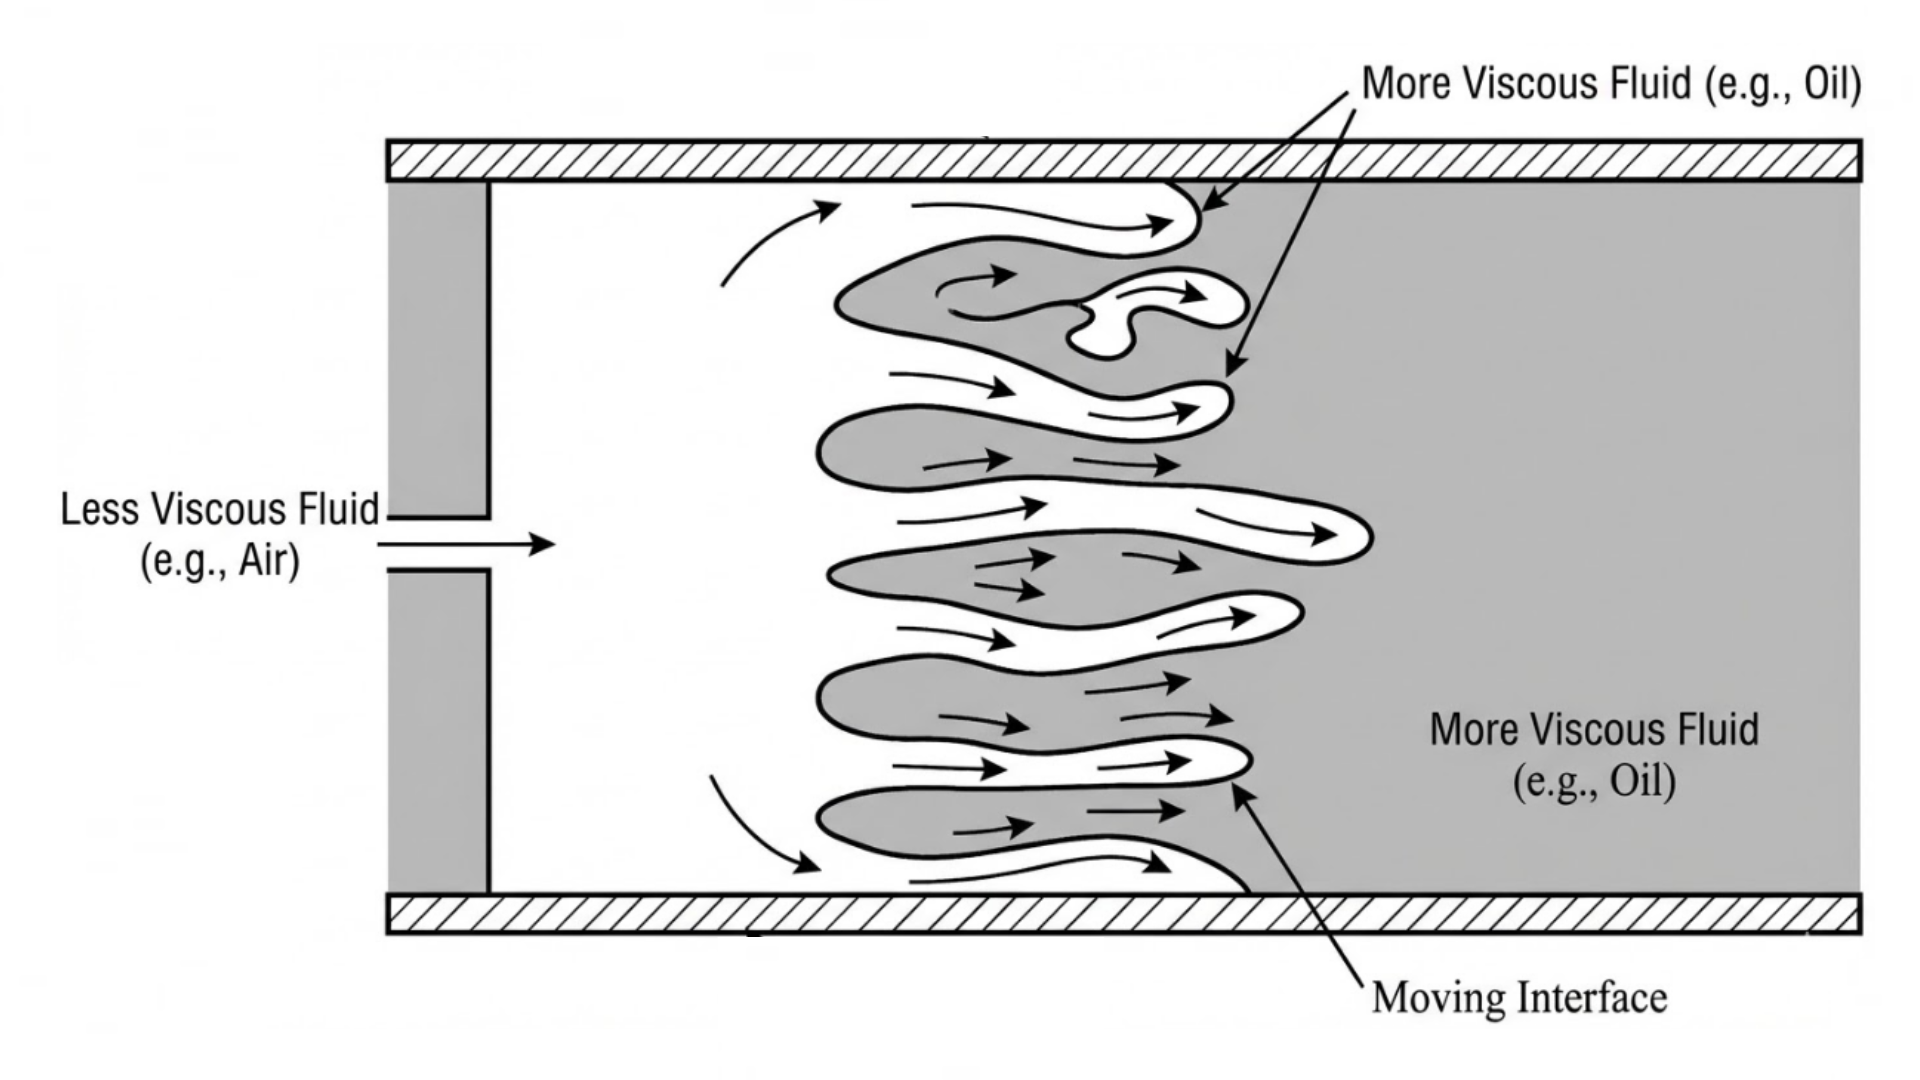
\includegraphics[width=0.8\linewidth]{figuras/introducao/fingering_example.png}
    \caption{Fingers patterns example}
    \label{fig:intro-saff-example}
\end{figure}


In the context of Enhanced Oil Recovery (EOR), the Saffman-Taylor instability acts as a  limiter to sweep efficiency. The propagation of viscous fingers leads to the premature breakthrough of the injected fluid at the production wells. Consequently, the water cut increases rapidly, leaving substantial volumes of bypassed, unrecoverable oil stranded within the reservoir matrix \cite{homsy1987viscous}. 

Various technological interventions have been developed to mitigate viscous fingering and improve the mobility ratio. Conventional chemical EOR strategies, such as polymer flooding, focus on increasing the apparent viscosity of the aqueous phase, thereby creating a more favorable mobility ratio and stabilizing the displacement front \cite{sheng2011modern}. More recent advancements involve the injection of foams, surfactants, and nanoparticle-stabilized emulsions (smart fluids) designed to alter interfacial tension and modify local rheology \cite{binks2002particles}. However, these approaches often face limitations regarding thermal degradation, mechanical shear degradation in the near-wellbore region, complex reservoir retention, and significant operational costs \cite{sorbie1991polymer, olajire2014review}.

To address these limitations, this study investigates a novel active-control mechanism: the application of magnetic fluids (ferrofluids) as the displacing phase. By exposing the injected magnetic fluid to an external magnetic field, an artificial body force (the Kelvin force) is induced at the fluid interface. Theoretical models and preliminary experiments demonstrate that a properly aligned magnetic field can counteract the hydrodynamic destabilization forces, effectively suppressing the Saffman-Taylor fingering \cite{jackson1993hydrodynamics, miranda1998radial}. 

Therefore, the primary objective of this thesis is the development and validation of a Computational Fluid Dynamics (CFD) simulation to model the multiphase displacement of oil by a magnetic fluid in a porous medium, supported by an analytical mathematical framework for theoretical validation. This computational framework will quantify the interfacial stabilization mechanisms and evaluate the sweep efficiency under varying magnetic field topologies and flow regimes.



%% FALAR O QUE É FLUIDO MAGNETICO 
%% QUANTIDADES DE PUBLICAÇÕES 
%% COMO AS PESSOAS ATACAM ESSES PROBLEMAS USUALMENTE
%% TEORIA PARA LEIGOS 
%% EXEMPLOS EXPERIMENTAIS DE SAFFMAN TAYLOR 